\documentclass{article}

\usepackage[preprint]{neurips_2026}

\usepackage[utf8]{inputenc}
\usepackage[T1]{fontenc}
\usepackage{hyperref}
\usepackage{url}
\usepackage{booktabs}
\usepackage{amsfonts}
\usepackage{nicefrac}
\usepackage{microtype}
\usepackage{xcolor}
\usepackage{graphicx}
\usepackage{placeins}

\title{DysXAI: Explainable AI for Dysgraphia Detection from Handwriting Kinematics}

\author{%
  Tia Manoukian \\
  Institut Polytechnique de Paris \\
  Master DataAI Research Project \\
  March 2026 \\
  \texttt{tia.manoukian@ip-paris.fr} \\
}


\begin{document}

\maketitle

\begin{abstract}
\textit{This paper presents DysXAI, an explainable deep learning pipeline designed to advance the automated detection of dysgraphia from digitized handwriting. Previous approaches using the Drotar dataset relied on aggregated summary statistics, an approach that unintentionally erases the fine-grained, millisecond-level details of a child's writing process. To solve this, DysXAI directly ingests raw, multivariate time-series data—spanning 13 kinematic channels—into three deep learning architectures: a 1D Convolutional Neural Network (CNN), a Temporal Convolutional Network (TCN), and a Hybrid CNN-LSTM. By analyzing the raw time-series, our models successfully capture micro-hesitations, sudden pressure changes, and high-frequency tremors as primary diagnostic signals. We evaluated these models using five repeated subject-independent splits with different seeds, as well as fixed hyperparameters and validation used only for early stopping and learning-rate scheduling. To rank clinical biomarkers, we applied a leakage-safe forward feature selection procedure on a single subject-independent train/validation/test partition (Phases~1--2 on train+validation; test held for Phase~3). This highlights confounds such as sequence length and age alongside raw feature importance. Ultimately, this work frames dysgraphia detection as more than just a classification problem. By exploring the future integration of counterfactual explanations (via TSInterpret and CoMTE), we demonstrate how Explainable AI can eventually transition this technology from a diagnostic tool into a prescriptive aid, providing occupational therapists with targeted insights for patient intervention.}
\end{abstract}


\section{Introduction}
\label{sec:intro}

Dysgraphia is a neurodevelopmental disorder affecting the acquisition and production of written language, characterized by difficulties in letter formation, spelling, and written expression~\cite{drotar2020}. It is frequently associated with other conditions such as dyslexia and developmental coordination disorder~\cite{drotar2020}. Importantly, dysgraphia is not associated with impaired intelligence; individuals typically possess at least average intelligence yet can be significantly hindered in academic progress and self-esteem when left undetected~\cite{kunhoth2022}. It affects approximately 5--15\% of school-aged children~\cite{american2013}. Traditional clinical testing relies primarily on static features (text shape, writing density) and manual scales (e.g., BHK in French, DASH in English), which are prone to subjective bias and resource-intensity~\cite{chung2019, kunhoth2024}.

Handwriting is a complex psychomotor skill involving fine motor control, neuromuscular coordination, and visuospatial functions. Shifting from static images to dynamic digital tablets---from the WACOM Intuos Pro tablet used in the Drotar dataset~\cite{drotar2020}---unlocks previously "invisible" spatiotemporal features, such as pen pressure, tilt, acceleration, on-air time, that are essential for objective, automated screening~\cite{drotar2020, kunhoth2022}. Recent work has applied machine learning to such data, achieving high accuracies (e.g., 76--88\% in~\cite{kunhoth2022, kunhoth2024multimodal}), but model interpretability remains limited, hindering clinical adoption and creating a trust gap in healthcare due to the "black box" nature of deep learning~\cite{asselborn2020, js2019ad}.

While Drotár and Dobeš \cite{drotar2020} successfully established the clinical value of tablet-captured handwriting dynamics, their methodology relied on aggregated scalar features paired with a traditional ensemble classifier (AdaBoost). This approach inherently discards critical sequential dynamics; the temporal ordering within a stroke, sub-stroke micro-variability, and the exact timing of hesitation pauses are lost when a dynamic writing trace is collapsed into a handful of summary statistics. DysXAI bridges this gap by directly ingesting raw, unaggregated multivariate time-series data into deep learning architectures. By transitioning to 1D convolutional (CNN), temporal convolutional (TCN), and hybrid recurrent (CNN-LSTM) networks, our pipeline captures localized, high-frequency patterns—such as micro-tremors, abrupt pressure drops, and millisecond-level hesitations—that global averages systematically mask.

We introduce DysXAI as a reproducible, explainability-aware pipeline designed to facilitate the clinical translation of automated dysgraphia screening. By pairing predictive outputs with interpretable feature-importance evidence, the framework aligns with broader diagnostic research in neurodevelopmental and neurodegenerative diseases \cite{js2019ad}. Our primary contributions are fivefold: (1) the implementation of a rigorous, subject-independent preprocessing and evaluation strategy on the Drotár corpus; (2) a comparative analysis of 1D CNN, TCN, and CNN-LSTM architectures under five repeated subject-independent splits; (3) a comprehensive error analysis contrasting unseen test-set performance with full-corpus evaluations; (4) a leakage-safe forward feature selection pipeline that ranks individual kinematic channels on a held-out validation set, superseding informal ablation; and (5) a theoretical framing of counterfactual explanations and gradient-based attributions (Deep SHAP) as future prescriptive tools for occupational therapists.


\section{Related Work}
\label{sec:related}

\subsection{From static diagnostics to dynamic kinematics}

Traditional clinical assessments for developmental dysgraphia---notably scales such as BHK (French) and DASH (English)---rely heavily on \textbf{static}, offline handwriting products and the rater's judgment, which can introduce subjective bias and limited reproducibility~\cite{chung2019, kunhoth2024}. Drot\'ar and Dobe\v{s}~\cite{drotar2020} helped catalyze a shift toward objective, data-driven screening by releasing a public corpus collected on a WACOM Intuos Pro tablet. Digitizing the writing trace unlocks "invisible" \textbf{spatiotemporal} signals---pen pressure, azimuth, altitude, and in-air movement---that static copies of handwriting do not preserve. Their pipeline aggregated a large hand-crafted feature space (on the order of \textbf{150+} statistical descriptors per task family) and trained AdaBoost, reporting approximately 80\% accuracy and an important clinical regularity: under \textbf{higher cognitive load} (e.g., the complex word \emph{hračkárstvo}), dysgraphic motor deficits become more pronounced~\cite{drotar2020}.

Subsequent work sought leaner feature sets that isolate robust biomarkers. Kunhoth et al.~\cite{kunhoth2022} showed that strong screening performance can be achieved with only \textbf{47} engineered features---far fewer than earlier high-dimensional pipelines of 150+ features. They identified \textbf{on-air time}---idle intervals between strokes that reflect planning, hesitation, and cognitive load---as the single most influential predictor, yielding roughly a \textbf{7.5\%} accuracy gain when included. Read alongside Drot\'ar and Dobe\v{s}~\cite{drotar2020}, this suggests a coherent narrative: difficult spelling--motor demands increase pausing and between-stroke structure, which discriminative models exploit. At the same time, Kunhoth et al.~\cite{kunhoth2022} caution that \textbf{writing velocity}, although informative in other handwriting-based diagnostics, is \textbf{strongly age-dependent} in pediatric cohorts since we are testing on ages between \textbf{8 snd 15}, and therefore a fragile standalone biomarker for dysgraphia screening across broad developmental ranges---a contrast with settings such as neurodegenerative disease, where kinematic slowing is often central~\cite{js2019ad}.


\subsection{Deep learning and multimodal paradigms}

Moving beyond the reliance on engineered scalar features, recent literature advocates for end-to-end learning directly from \textbf{raw time-series data} to prevent the premature collapse of temporal micro-structures. Masood et al.~\cite{masood2023} introduced a hybrid CNN-LSTM architecture for handwritten character classification. In their approach, convolutional blocks act as feature extractors for local stroke-level patterns, while recurrent layers model longer-range temporal dependencies.  This methodology directly motivates the hybrid sequence architecture evaluated in our pipeline, which we have adapted specifically for multichannel tablet sequences and strictly subject-independent evaluation.

Concurrently, the field is advancing toward multimodal protocols that jointly analyze both the product (static images) and the process (online kinematics) of writing. Kunhoth et al.~\cite{kunhoth2024multimodal} demonstrated strong diagnostic capabilities, achieving 88.8\% accuracy using an Ensemble with Conditional Feature Fusion (ECFF). This system routes uncertain predictions through a secondary decision pathway, illustrating that structured modality fusion can enhance classification robustness just as effectively as increasing network depth. Looking forward, a recent survey by Kunhoth et al.~\cite{kunhoth2024} argues that comprehensively addressing the five distinct subtypes of dysgraphia will ultimately require richer sensing modalities. Incorporating surface electromyography (sEMG) and force-sensitive resistors into the writing instrument could capture grip forces and proximal muscle coordination, providing critical biomechanical context that standard digitizing tablets inherently omit. We leave this for future studies.

\subsection{Explainable AI (XAI) in healthcare and time-series settings}

Despite strong accuracy, deep pipelines risk a \textbf{trust gap}: clinicians need rationales that map model behavior to measurable kinematic quantities~\cite{arrieta2020, js2019ad}. For Alzheimer's detection from \textbf{online} handwriting, Sweidan et al.~\cite{js2019ad} combined gradient attributions (\textbf{DeepSHAP}), temporal saliency rescaling (\textbf{TSR}), and \textbf{counterfactual} explanations (CoMTE)}to articulate not only which features matter, but what magnitude of change in the trace would move a case toward a "healthier" decision boundary---a step toward prescriptive, therapist-actionable narratives.


\section{Methods}
\label{sec:methods}

\subsection{Dataset and Preprocessing}

We use the public Drotar dataset~\cite{drotar2020} from Scientific Reports, notably handwriting samples from 120 subjects, 57 being dysgraphic and 63 control or non-dysgraphic. These samples were collected on a WACOM Intuos Pro Large tablet capturing pen movement (x, y), pressure, azimuth, altitude, and pen-on-surface status. Each sample is a multi-channel time-series with 7 base channels: x, y, time, pressure, azimuth, altitude, pen\_status. Additionally, I compute 6 derivative features---velocity (vx, vy), acceleration (ax, ay), and jerk (jx, jy)---yielding 13 input channels, consistent with prior work emphasizing kinematic features~\cite{drotar2020, kunhoth2022}. Sequences are padded or truncated to 2000 time steps.

\paragraph{Mixed feature scaling and leakage prevention.} To ensure numerical stability without distorting clinically meaningful biomarkers, we implement a mixed feature scaling strategy. To strictly prevent data leakage, all scaling parameters are computed exclusively on the training folds before being applied to the validation and test sets. Spatial coordinates ($X$ and $Y$) are transformed using global Min-Max scaling based on the training set boundaries. This approach preserves the relative geometry, aspect ratio, and bounding-box proportions of the handwriting trace while mapping varying tablet coordinate spaces to a uniform numeric scale. Conversely, kinematic and physical channels (e.g., pressure, velocity, acceleration, jerk, and pen tilt) are standardized to zero mean and unit variance. This ensures that the network optimization is not disproportionately dominated by naturally high-variance channels. 

Data are split by \textbf{subject ID} in a strict 3-way split (70\% train, 15\% validation, 15\% test) so no subject appears in multiple splits, which is critical for generalization and avoiding leakage.

\subsection{Model Architectures}

The study evaluates three distinct sequence-modeling architectures. The \textbf{1D Convolutional Neural Network (CNN)} comprises three sequential convolutional blocks with progressively increasing filters (64, 128, and 256 channels) and decreasing kernel sizes (7, 5, and 3, respectively). Each block incorporates batch normalization, ReLU activation, and max pooling, culminating in a masked global average pooling layer and a binary classification head. Alternatively, the \textbf{Temporal Convolutional Network (TCN)} employs dilated causal convolutions paired with residual connections to effectively capture long-range temporal dependencies while strictly preventing future-data leakage.

Finally, inspired by Masood et al.~\cite{masood2023}, the \textbf{hybrid CNN-LSTM} architecture utilizes two convolutional layers (64 and 128 channels) for localized spatial-temporal feature extraction. These feature maps are subsequently fed into a two-layer bidirectional LSTM (with a hidden size of 64) equipped with dropout to model complex sequential patterns. To mitigate dataset imbalance and prevent overfitting, all three models are trained using class-weighted cross-entropy loss and incorporate an early stopping mechanism that monitors validation loss with a patience of five epochs.

\subsection{Evaluation Protocol}

We evaluate all architectures across five repeated, subject-independent data splits (random seeds 42, 123, 456, 789, and 1011). Hyperparameters are \textbf{fixed} across runs (not tuned via nested cross-validation). Within each split, the mixed feature scaler is fit on training subjects only. The validation set is used solely for early stopping and \texttt{ReduceLROnPlateau} scheduling; the test set is held out until the final evaluation. We report \textbf{accuracy, sensitivity, specificity, and AUC} as mean $\pm$ standard deviation across the five runs.

\subsection{Test vs.\ full-corpus confusion matrices}

For each architecture, we report two confusion matrices from the same final split run: (i) the held-out \textbf{test} set (15\% of subjects); (ii) the \textbf{full} corpus ($N{=}121$ samples; 120 subjects). The latter reuses training and validation data and therefore does not estimate generalization; it supports qualitative error patterns alongside the test matrix.

\section{Experiments}
\label{sec:experiments}

\subsection{Implementation and setup}

All architectures were trained using the Adam optimizer with an initial learning rate of $10^{-3}$ and a weight decay of $10^{-4}$ to apply $L_2$ regularization. Network training was conducted over a maximum of $50$ epochs with a batch size of $16$. To address the inherent class imbalance within the clinical cohort, we utilized class-weighted cross-entropy loss during the optimization phase. Furthermore, a learning rate scheduler (\texttt{ReduceLROnPlateau}) was implemented to dynamically reduce the learning rate if the validation loss stagnated, ensuring finer convergence. The entire experimental pipeline was modularized into distinct, reproducible stages encompassing data initialization, isolated model training, forward feature selection, and explainability analysis.

\subsection{Main quantitative results}

Tables~\ref{tab:results-cnn1d}--\ref{tab:results-cnnlstm} report test-set metrics per run and aggregated mean $\pm$ standard deviation (Section~\ref{sec:methods}).

\begin{table}[ht]
  \caption{\textbf{1D CNN}: test-set metrics per run and mean $\pm$ standard deviation over five splits.}
  \label{tab:results-cnn1d}
  \centering
  \footnotesize
  \setlength{\tabcolsep}{4pt}
  \begin{tabular}{l ccccc c}
    \toprule
    Metric & Run 1 & Run 2 & Run 3 & Run 4 & Run 5 & Mean $\pm$ Std \\
    \midrule
    Accuracy    & 0.8889 & 0.8889 & 1.0000 & 0.8333 & 1.0000 & $0.9222 \pm 0.0667$ \\
    Sensitivity & 0.7778 & 0.8750 & 1.0000 & 0.7000 & 1.0000 & $0.8706 \pm 0.1194$ \\
    Specificity & 1.0000 & 0.9000 & 1.0000 & 1.0000 & 1.0000 & $0.9800 \pm 0.0400$ \\
    AUC         & 0.9753 & 0.9875 & 1.0000 & 0.8625 & 1.0000 & $0.9651 \pm 0.0521$ \\
    \bottomrule
  \end{tabular}
\end{table}

\begin{table}[ht]
  \caption{\textbf{TCN}: test-set metrics per run and mean $\pm$ standard deviation over five splits.}
  \label{tab:results-tcn}
  \centering
  \footnotesize
  \setlength{\tabcolsep}{4pt}
  \begin{tabular}{l ccccc c}
    \toprule
    Metric & Run 1 & Run 2 & Run 3 & Run 4 & Run 5 & Mean $\pm$ Std \\
    \midrule
    Accuracy    & 0.8333 & 0.9444 & 0.9444 & 0.8889 & 1.0000 & $0.9222 \pm 0.0567$ \\
    Sensitivity & 0.7778 & 0.8750 & 1.0000 & 0.8000 & 1.0000 & $0.8906 \pm 0.0950$ \\
    Specificity & 0.8889 & 1.0000 & 0.8571 & 1.0000 & 1.0000 & $0.9492 \pm 0.0630$ \\
    AUC         & 0.9753 & 0.9750 & 1.0000 & 0.8750 & 1.0000 & $0.9651 \pm 0.0464$ \\
    \bottomrule
  \end{tabular}
\end{table}

\begin{table}[ht]
  \caption{\textbf{CNN--LSTM}: test metrics per run and mean $\pm$ standard deviation over five subject-independent splits.}
  \label{tab:results-cnnlstm}
  \centering
  \footnotesize
  \setlength{\tabcolsep}{4pt}
  \begin{tabular}{l ccccc c}
    \toprule
    Metric & Run 1 & Run 2 & Run 3 & Run 4 & Run 5 & Mean $\pm$ Std \\
    \midrule
    Accuracy    & 0.8333 & 0.8889 & 0.9444 & 0.8889 & 1.0000 & $0.9111 \pm 0.0567$ \\
    Sensitivity & 0.7778 & 0.7500 & 1.0000 & 0.8000 & 1.0000 & $0.8656 \pm 0.1109$ \\
    Specificity & 0.8889 & 1.0000 & 0.8571 & 1.0000 & 1.0000 & $0.9492 \pm 0.0630$ \\
    AUC         & 0.8889 & 0.9500 & 0.9610 & 0.8500 & 1.0000 & $0.9300 \pm 0.0536$ \\
    \bottomrule
  \end{tabular}
\end{table}

\textbf{Cross-model summary.} In this experiment log, 1D CNN and TCN share the highest mean test accuracy and mean AUC ($0.9222$ and $0.9651$). While the hybrid CNN--LSTM attains mean accuracy $0.9111 \pm 0.0567$ and mean AUC $0.9300 \pm 0.0536$---slightly lower on average, with sensitivity and specificity spreads comparable in magnitude to the other architectures.

\paragraph{Channel salience and feature ranking.}
Phase~1 isolates each channel on the \textbf{validation} set of a single subject-independent split (Section~\ref{sec:explainability}); rankings appear in Table~\ref{tab:phase1}.


\subsection{Architectural comparison: localized CNN versus hybrid CNN--LSTM}
Counterintuitively, the relatively localized 1D CNN architecture demonstrates performance that matches or exceeds that of the more complex hybrid CNN--LSTM within our experimental framework. While bidirectional LSTMs are theoretically well-suited for modeling long-range temporal structures, their high parameter density significantly increases model variance when training data is limited. Given the restricted size of the clinical cohort of 120 subjects, deep recurrent networks are highly susceptible to overfitting to the particular writing styles of the training subjects rather than learning generalizable dysgraphic signatures. Conversely, the 1D CNN acts as an aggressive local feature extractor. Its inductive bias favors short receptive fields that are optimally aligned with high-frequency kinematic anomalies, such as sudden pressure drops, velocity spikes, and jerk transients. This performance discrepancy suggests that, for this specific clinical task, discriminative evidence is predominantly concentrated in localized motor irregularities rather than in the slow, macro-level evolution of the full handwriting sequence. These findings offer a compelling hypothesis regarding the nature of dysgraphic biomarkers, though they warrant further validation on larger, age-balanced corpora.

\subsection{Training dynamics and loss convergence}
Figure~\ref{fig:loss-all} shows train and validation loss, averaged over the five repeated splits (shaded: $\pm$ std). Early stopping on validation loss and \texttt{ReduceLROnPlateau} limit overfitting relative to training loss alone.

\begin{figure}[!htbp]
  \centering
  \begin{minipage}{\linewidth}
    \centering
    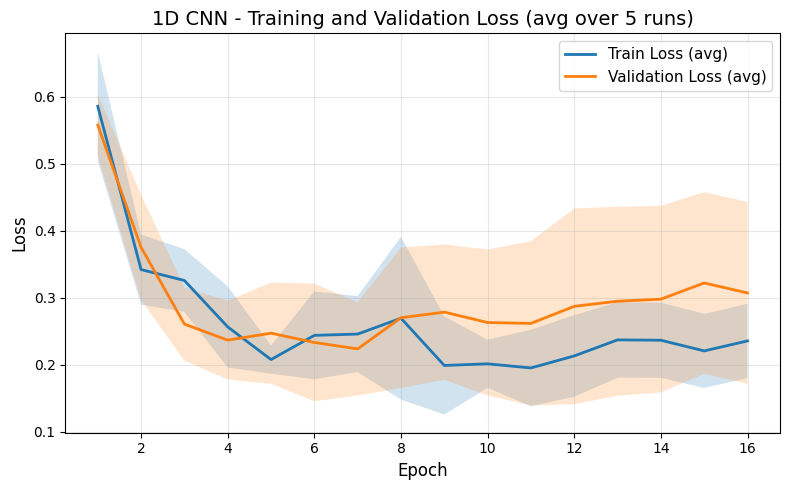
\includegraphics[width=0.85\linewidth]{figures/fig_cnn1d_loss.png}
    \\[0.35em]
    \small (a) 1D CNN
  \end{minipage}

  \vspace{0.85em}

  \begin{minipage}{\linewidth}
    \centering
    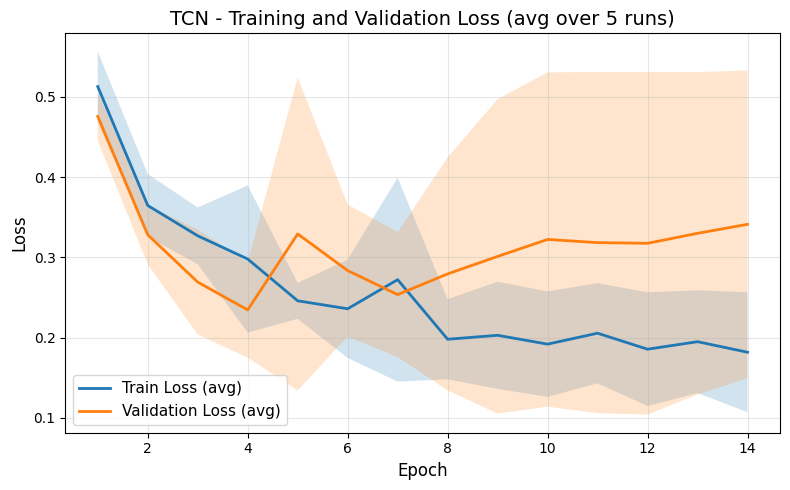
\includegraphics[width=0.85\linewidth]{figures/fig_tcn_loss.png}
    \\[0.35em]
    \small (b) TCN
  \end{minipage}

  \vspace{0.85em}

  \begin{minipage}{\linewidth}
    \centering
    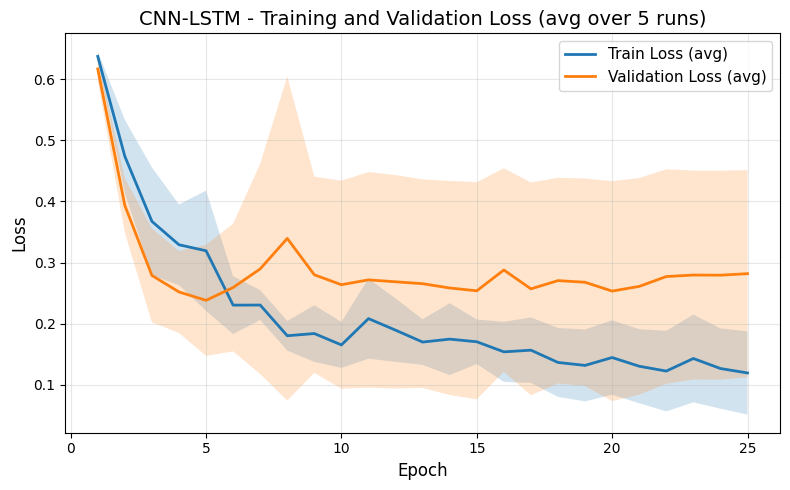
\includegraphics[width=0.85\linewidth]{figures/fig_cnnlstm_loss.png}
    \\[0.35em]
    \small (c) CNN-LSTM
  \end{minipage}
  \caption{Training and validation loss (preferred: average $\pm$ std over five runs).}
  \label{fig:loss-all}
\end{figure}
\FloatBarrier


\subsection{Confusion matrices (test and full corpus)}
\label{subsec:confusion_matrices}

Figures~\ref{fig:cm-cnn1d}--\ref{fig:cm-cnnlstm} show test vs.\ full-corpus matrices per architecture (same protocol as Section~\ref{sec:methods}).

\begin{figure}[ht]
  \centering
  \begin{minipage}[b]{0.48\textwidth}
    \centering
    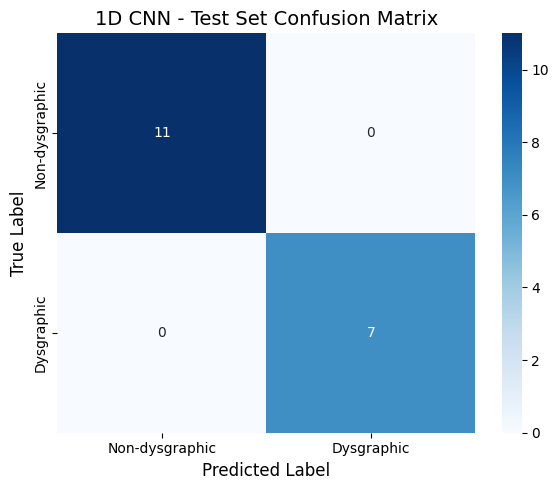
\includegraphics[width=\linewidth]{figures/fig_cnn1d_cm_test.png}
    \\[0.3em]
    \small (a) Test set (last run)
  \end{minipage}
  \hfill
  \begin{minipage}[b]{0.48\textwidth}
    \centering
    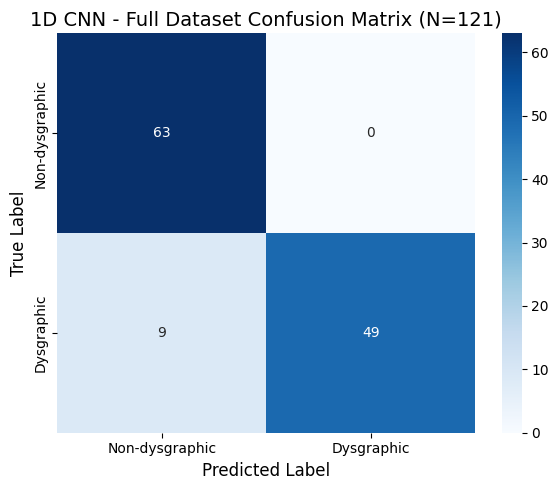
\includegraphics[width=\linewidth]{figures/fig_cnn1d_cm_full.png}
    \\[0.3em]
    \small (b) Full dataset ($N{=}121$, same run; not held-out)
  \end{minipage}
  \caption{1D CNN: test vs.\ full-corpus confusion matrices.}
  \label{fig:cm-cnn1d}
\end{figure}

\begin{figure}[ht]
  \centering
  \begin{minipage}[b]{0.48\textwidth}
    \centering
    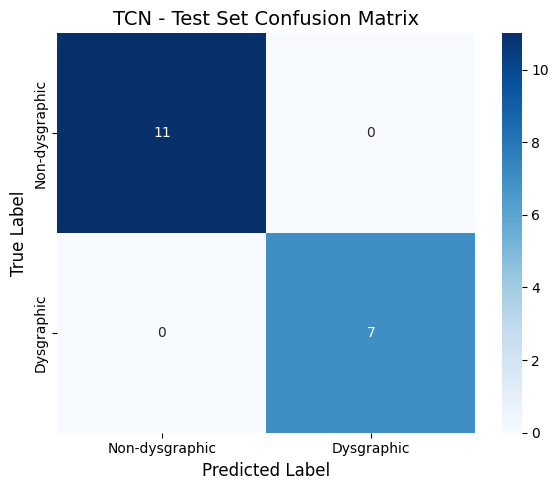
\includegraphics[width=\linewidth]{figures/fig_tcn_cm_test.png}
    \\[0.3em]
    \small (a) TCN --- test set
  \end{minipage}
  \hfill
  \begin{minipage}[b]{0.48\textwidth}
    \centering
    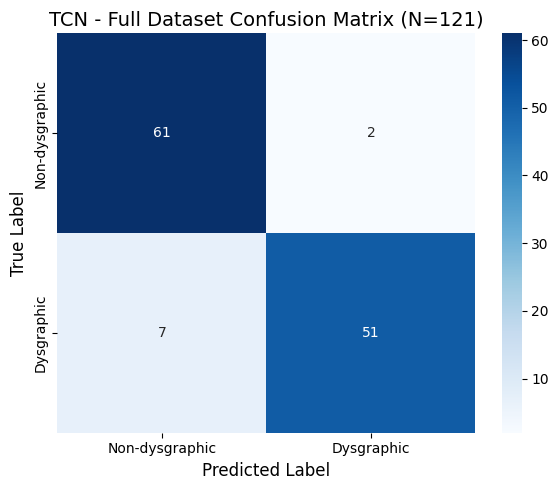
\includegraphics[width=\linewidth]{figures/fig_tcn_cm_full.png}
    \\[0.3em]
    \small (b) TCN --- full dataset
  \end{minipage}
  \caption{TCN confusion matrices.}
  \label{fig:cm-tcn}
\end{figure}

\begin{figure}[ht]
  \centering
  \begin{minipage}[b]{0.48\textwidth}
    \centering
    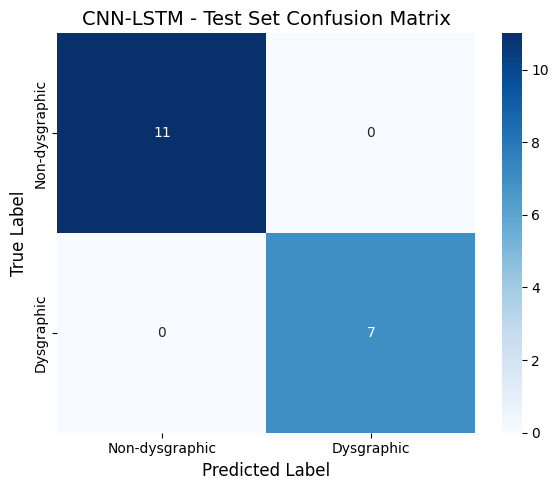
\includegraphics[width=\linewidth]{figures/fig_cnnlstm_cm_test.png}
    \\[0.3em]
    \small (a) CNN-LSTM --- test set
  \end{minipage}
  \hfill
  \begin{minipage}[b]{0.48\textwidth}
    \centering
    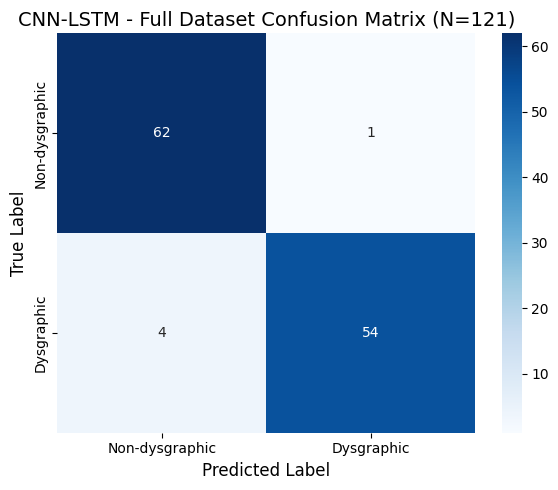
\includegraphics[width=\linewidth]{figures/fig_cnnlstm_cm_full.png}
    \\[0.3em]
    \small (b) CNN-LSTM --- full dataset
  \end{minipage}
  \caption{CNN-LSTM confusion matrices.}
  \label{fig:cm-cnnlstm}
\end{figure}

The confusion matrices provide a granular view of model performance, distinguishing between strict generalization and overall cohort fit. For the \textbf{1D CNN} (Figure~\ref{fig:cm-cnn1d}), the isolated test set shows perfect classification for the held-out subjects ($N=18$), with 11 non-dysgraphic and 7 dysgraphic subjects correctly identified. When observing the \textbf{full-corpus matrix}, which includes the training and validation subsets, the model correctly classifies 112 out of 121 total subjects.  However, the presence of 9 false negatives---dysgraphic children misclassified as non-dysgraphic---highlights a specific area for clinical improvement. This gap suggests that while the model captures high-frequency kinematic anomalies, some subtle dysgraphic signatures in the training set remain challenging to distinguish from typical writing variability. Comparable patterns are observed for the \textbf{TCN} (Figure~\ref{fig:cm-tcn}), which correctly identifies all 7 dysgraphic subjects in the test set but shows a slight decrease in false negatives (7 subjects) across the full dataset compared to the 1D CNN, but we have 2 cases of false positives. Finally, the \textbf{CNN-LSTM} architecture (Figure~\ref{fig:cm-cnnlstm}) matches the 1D CNN's perfect test-set performance ($N=18$) but demonstrates the lowest number of false negatives in the full-corpus evaluation ($N=4$), and 1 false positive.

\section{Explainability Analysis}
\label{sec:explainability}

To support clinical translation, we connect our evidence to quantities that occupational therapists (OTs) can readily interpret: timing, pressure, pen orientation, and kinematics along each axis. Instead of standard horizontal bar plots (e.g., test AUC drop under channel zeroing), we report the Phase 1 isolated-channel validation performance in table~\ref{tab:phase1}. This approach ranks the informativeness of each channel when the model evaluates it in isolation ~\cite{arrieta2020}.

\subsection{Phase~1 channel ranking }

In Phase 1, a 1D Convolutional Neural Network (CNN) is trained using one channel at a time. The features are then ranked according to their validation Area Under the Curve (AUC), with accuracy serving as a tie-breaker. As detailed in table~\ref{tab:phase1}, kinematic features such as Velocity X, Acceleration Y, Acceleration X, and Velocity Y rank immediately after Time in terms of predictive performance. Conversely, raw X and Y positional coordinates rank lowest. These results indicate that, in this specific experimental setup, kinematic dynamics provide more discriminative structural information than spatial coordinates alone.

\paragraph{Unexpected prominence of \textbf{Time} vs.\ the literature.} The logged Phase~1 run places the raw \textbf{Time} stamp channel first, with validation AUC effectively perfect---an outcome we consider \textbf{unexpected} and potentially \textbf{misleading} without further checks. Prior work on similar tablet corpora highlights \textbf{on-air time} (idle time between strokes, reflecting cognitive and motor planning load) as a dominant hand-crafted predictor~\cite{kunhoth2022}, not a monotonic clock channel fed to a deep model. In our pipeline, \textbf{Time} indexes the resampled/padded sequence; the network may exploit \textbf{gross writing duration}, effective sequence length after padding, tempo, or confounds such as \textbf{age} rather than clinically specific pause structure. This tension between our ranking and the on-air-time literature is discussed further in Section~\ref{sec:discussion}, together with planned analyses we have not yet run.

\begin{table}[ht]
  \caption{Phase~1 ranked channels (isolated-channel 1D CNN).}
  \label{tab:phase1}
  \centering
  \footnotesize
  \begin{tabular}{r l cc}
    \toprule
    Rank & Feature & Val.\ AUC & Val.\ Acc. \\
    \midrule
    1  & Time            & 1.0000 & 0.9444 \\
    2  & Velocity\_X     & 0.9750 & 0.9444 \\
    3  & Acceleration\_Y & 0.9750 & 0.9444 \\
    4  & Acceleration\_X & 0.9750 & 0.8889 \\
    5  & Velocity\_Y     & 0.9500 & 0.9444 \\
    6  & Jerk\_X         & 0.8875 & 0.8889 \\
    7  & Jerk\_Y         & 0.8750 & 0.9444 \\
    8  & Azimuth         & 0.8000 & 0.7222 \\
    9  & Pressure        & 0.7500 & 0.5556 \\
    10 & Pen\_Status     & 0.7500 & 0.4444 \\
    11 & Altitude        & 0.5750 & 0.5000 \\
    12 & Y               & 0.5625 & 0.5556 \\
    13 & X               & 0.1375 & 0.5556 \\
    \bottomrule
  \end{tabular}
\end{table}

\subsection{Forward feature selection (Phases 2--3)}

Beyond Phase~1 (Table~\ref{tab:phase1}), we run greedy forward addition on one subject-independent 70/15/15 split: Phases~1--2 use train and validation only; the test set is evaluated \textbf{once} in Phase~3. This is not $k$-fold cross-validation over multiple partitions, but strict train/val/test isolation to avoid test leakage during selection. 


\subsection{Counterfactual explanations (intent and future work)}

Beyond feature attribution, multivariate \textbf{counterfactual} methods (e.g., CoMTE via TSInterpret~\cite{tsinterpret}, as explored for Alzheimer's handwriting~\cite{js2019ad}) aim to answer: \emph{what minimal change to the time series would flip the prediction?} For dysgraphia screening, such outputs could move the system from purely \textbf{diagnostic} ("dysgraphic vs.\ control") toward \textbf{prescriptive} support: Therapists could review suggested perturbation patterns---conceptually, e.g.\ reduced variance in pen pressure or smoother vertical velocity profiles---as \textbf{actionable} training targets, always subject to clinical judgment. 


\section{Discussion}
\label{sec:discussion}

\textbf{Limitations (cohort and evaluation).} The public corpus is small (121 samples; 120 subjects). Performance on other tablets, languages, or age groups may differ. Full-corpus confusion matrices are useful for diagnostics but overstate certainty compared to subject-held-out test metrics. \textbf{X/Y scaling} may hide micrographia/macrographia; alternative normalizations deserve study.

\textbf{Age as a primary confounder.} A central limitation of time-series handwriting analysis on developmental cohorts is \textbf{age}: the Drotar release spans children roughly 8--15 years, an interval of rapid motor maturation. Older children tend to write faster and produce shorter task durations for the same stimulus, while base velocity and jerk profiles shift with neuromuscular development. Consequently, strong Phase~1 scores for \textbf{Time} and \textbf{Velocity} (Table~\ref{tab:phase1}) may partly reflect \textbf{age stratification} rather than dysgraphia-specific hesitation alone. Future work must disentangle these effects via \textbf{age-stratified} training/evaluation, inclusion of age as a covariate, or matching, and via features that isolate within-writer pause structure independent of gross sequence length.

\textbf{Interpretation of Time and follow-up (future work).} 
Time appears overwhelmingly informative in Phase 1. To determine if this reflects true dysgraphic slowing rather than sequence length confounding, I plan to implement several analytical steps suggested by Dr. El Yacoubi. We will derive total task duration from raw tablet timestamps (decoupled from model padding) and compare the distributions of these durations between dysgraphic and control groups using kernel density estimates or histograms.  Characterizing the overlap and effect size between these groups will establish whether gross duration is a reliable biomarker. Substantial overlap would motivate literature-backed features such as on-air intervals or within-task pauses~\cite{kunhoth2022}. Until this analysis is complete, the high predictive rank of Time must be treated as a potential warning flag for length-based confounding rather than clinical evidence of slow writing.

\textbf{Broader impact.} Screening tools should augment, not replace, clinical judgment. Explainability is intended to support transparent review of model behavior for clinicians and families.

\section{Conclusion}
\label{sec:conclusion}

DysXAI advances beyond the classical Drotar pipeline by demonstrating the efficacy of end-to-end learning on raw multivariate traces. Comparing 1D CNN, TCN, and CNN-LSTM models via subject-independent splits reveals a practical trade-off between localized and recurrent architectures for small clinical datasets. This work also establishes a leakage-safe scaling methodology and leverages Phase 1 forward selection for initial interpretability.

Future work will prioritize the timestamp-based duration and group overlap analyses outlined by Dr. El Yacoubi. Subsequent steps include applying Deep SHAP for advanced multichannel ablation, integrating age-aware metrics (as done by Jihyun Mun), and utilizing established on-air/pause features. The ultimate goal remains the development of stable counterfactuals to provide occupational therapists with highly prescriptive and interpretable clinical summaries.

\begin{ack}
  I conducted this Master's research project with the very helpful guidance of Dr.\ Mounim El Yacoubi, along with Jihyun Mun and Jana Sweidan who work in his research team. 
  
\end{ack}

\section*{References}

\begin{thebibliography}{12}

\bibitem{drotar2020}
Drot\'ar, P., and Dobe\v{s}, M. (2020).
\newblock Dysgraphia detection through machine learning.
\newblock \textit{Scientific Reports}, \textbf{10}, 21541.
\newblock DOI: \href{https://doi.org/10.1038/s41598-020-78611-9}{10.1038/s41598-020-78611-9}.

\bibitem{asselborn2020}
Asselborn, T., Chapatte, M., and Dillenbourg, P. (2020).
\newblock Automated human-level diagnosis of dysgraphia using a consumer tablet.
\newblock \textit{npj Digital Medicine}, 3:97.

\bibitem{american2013}
American Psychiatric Association (2013).
\newblock \textit{Diagnostic and Statistical Manual of Mental Disorders} (5th ed.).

\bibitem{arrieta2020}
Arrieta, A.~B., Diaz-Rodriguez, N., and Del Ser, J. (2020).
\newblock Explainable Artificial Intelligence (XAI): Concepts, taxonomies, opportunities.
\newblock \textit{Information Fusion}, 58:82--115.

\bibitem{chung2019}
Chung, P.~J., Patel, D.~R., and Nizami, I. (2019).
\newblock Disorder of written expression and dysgraphia: Overview and framework for research.
\newblock \textit{Cognitive Neuropsychology}.

\bibitem{masood2023}
Masood, F., Khan, W.~U., Ullah, K., et al. (2023).
\newblock Hybrid CNN-LSTM random forest model for dysgraphia classification from hand-written characters.
\newblock \textit{Applied Sciences}, 13(7):4275. MDPI.

\bibitem{kunhoth2022}
Kunhoth, J., Al Maadeed, S., Saleh, M., and Akbari, Y. (2022).
\newblock Machine learning methods for dysgraphia screening with online handwriting features.
\newblock Qatar University. On-air time most critical; velocity age-dependent.

\bibitem{kunhoth2024}
Kunhoth, J., Al-Maadeed, S., Kunhoth, S., Akbari, Y., and Saleh, M. (2024).
\newblock Automated systems for diagnosis of dysgraphia in children: A survey and novel framework.
\newblock Five dysgraphia subtypes; multimodal future with sEMG, FSR.

\bibitem{kunhoth2024multimodal}
Kunhoth, J., Al Maadeed, S., Saleh, M., and Akbari, Y. (2024).
\newblock Multimodal ensemble with conditional feature fusion for dysgraphia diagnosis in children.
\newblock ECFF achieves 88.8\%; single-instance efficiency.

\bibitem{js2019ad}
Sweidan, A., El-Yacoubi, M.~A., and Rigaud, A.-S. (2019).
\newblock Explainability of CNN-based Alzheimer's disease detection from online handwriting.
\newblock \textit{Journal}. DeepSHAP, TSR, CoMTE counterfactuals for clinical trust.

\bibitem{tsinterpret}
Höllig, J., Kulbach, C., and Thoma, S. (2022).
\newblock TSInterpret: A unified framework for time series interpretability.
\newblock CoMTE, TSEvo, NUN-CF, TSR, LEFTIST; PyTorch/TensorFlow support.

\end{thebibliography}

\end{document}
